\chapter{Double Integrals Over Non-Rectangular Regions}


Now that we've seen how to evaluate double integrals over rectangular regions, 
let's consider non-rectangular regions. Suppose we are interested in the 
integral of a function, $f(x,y)$, over a region, \textit{D}, exists such that 
it can be bounded by inside a rectangular region, \textit{R} (see figure 
\ref{fig:enclose}). We can then define a new function:
$$F(x, y) = 
\begin{cases}
	f(x, y) & \text{if } (x, y) \text{ is in \textit{D}}\\
	0 & \text{if } (x, y) \text{ is in \textit{R} but not in \textit{D}}
\end{cases}$$

\begin{figure}[htbp]
    \centering
    \begin{minipage}{0.45\textwidth}
        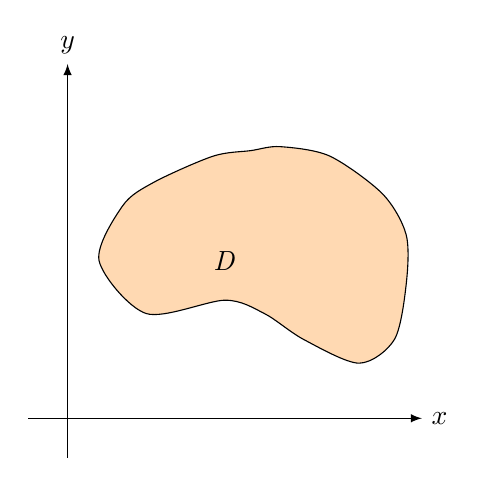
\begin{tikzpicture}
            \draw[-latex] (-0.5, 0) -- (4.5, 0) node[right] {$x$};
            \draw[-latex] (0, -0.5) -- (0, 4.5) node[above] {$y$};
            \draw[fill = orange!30] plot [smooth cycle] 
        coordinates {(0.4, 2) (0.7, 2.7) (1.1, 3) (1.85, 3.33) (2.33, 3.4) 
        (2.7, 3.45) (3.33, 3.33) (4, 2.85) (4.3, 2.33) (4.3, 1.7) (4.15, 1) 
        (3.7, 0.7) (3, 1) (2.5, 1.33) (2, 1.5) (1, 1.33)};
        \node[] at (2, 2) {\textit{D}};
        \end{tikzpicture}
    \end{minipage}
    \begin{minipage}{0.45\textwidth}
        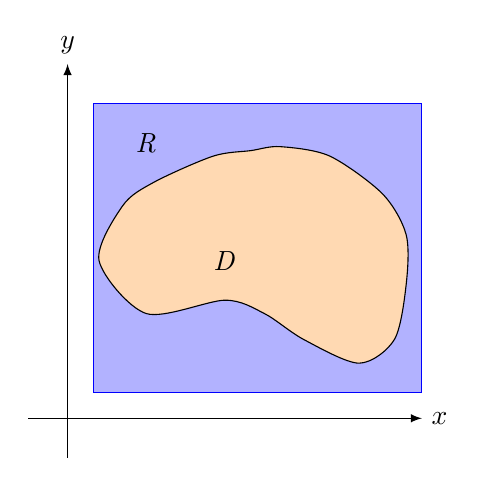
\begin{tikzpicture}
            \draw[-latex] (-0.5, 0) -- (4.5, 0) node[right] {$x$};
            \draw[-latex] (0, -0.5) -- (0, 4.5) node[above] {$y$};
            \draw[blue, fill = blue!30] (0.33, 0.33) rectangle (4.5, 4);
            \draw[fill = orange!30] plot [smooth cycle] 
        coordinates {(0.4, 2) (0.7, 2.7) (1.1, 3) (1.85, 3.33) (2.33, 3.4) 
        (2.7, 3.45) (3.33, 3.33) (4, 2.85) (4.3, 2.33) (4.3, 1.7) (4.15, 1) 
        (3.7, 0.7) (3, 1) (2.5, 1.33) (2, 1.5) (1, 1.33)};
        \node[] at (2, 2) {\textit{D}};
        \node[] at (1, 3.5) {\textit{R}};
        \end{tikzpicture}
    \end{minipage}
    \caption{We can find a rectangular region, \textit{R}, that completely 
    encloses \textit{D}}
    \label{fig:enclose}
\end{figure}

Then, we can see that:
$$\iint_{\textit{D}} f(x, y)\,dA = \iint_{\textit{R}} F(x, y)\,dA$$

Which makes sense intuitively, since integrating over $F$ outside of \textit{D}
doesn't contribute anything to the integral, and the integral of $F$ inside 
\textit{D} is equal to the integral of $f$ inside \textit{D}. In general, there
are two types of regions for \textit{D}. A region is \textbf{type I} if it lies
between two continuous functions of $x$ and can be defined thusly:
$$\textit{D} = \{ (x, y) \text{ } | \text{ } a \leq x \leq b, g_1(x) \leq y 
\leq g_2(x) \}$$

\begin{figure}[htbp]
    \centering
    \begin{minipage}{0.5\textwidth}
        \begin{tikzpicture}
            \begin{axis}[ymin = -0.3, ymax = 4, xmin = -0.3, xmax = 3, 
            axis lines = center, ticks = none, xlabel = $x$, ylabel = $y$] 
                \addplot[name path = A, domain = 0.5:2.5, orange, thick] {
                (0.5*x - 0.75)^2 + 0.5};
                \addplot[name path = B, domain = 0.5:2.5, orange, thick] {
                (x-2)^3 + 2*(x-2)^2 + x -1 + 1.5};
                \addplot[fill = orange!30] fill between [of = A and B];
                \draw[orange, thick] (0.5, 0.75) -- (0.5, 2.12);
                \draw[orange, thick] (2.5, 0.75) -- (2.5, 3.65);
                \draw[dashed] (0.5, 0.75) -- (0.5, 0) node[below] {$a$};
                \draw[dashed] (2.5, 0.75) -- (2.5, 0) node[below] {$b$};
                \node[] at (1.5, 2.8) {$y = g_2 (x)$};
                \node[] at (1.75, 0.25) {$y = g_1 (x)$};
                \node[] at (1.5, 1.5) {\textit{D}};
            \end{axis}
        \end{tikzpicture}
    \end{minipage}
    
    \begin{minipage}{0.5\textwidth}
        \begin{tikzpicture}
            \begin{axis}[ymin = -0.3, ymax = 4, xmin = -0.3, xmax = 3, 
            axis lines = center, ticks = none, xlabel = $x$, ylabel = $y$] 
                \addplot[name path = A, domain = 0.5:2.5, orange, thick, 
                samples = 150] {1.75 + sqrt(x - 0.5)};
                \addplot[name path = B, domain = 0.5:2.5, orange, thick, 
                samples = 150] {1.75 - sqrt(x - 0.5)};
                \addplot[fill = orange!30] fill between [of = A and B];
                \draw[orange, thick] (2.5, 0.33) -- (2.5, 3.17);
                \draw[dashed] (0.5, 1.75) -- (0.5, 0) node[below] {$a$};
                \draw[dashed] (2.5, 0.33) -- (2.5, 0) node[below] {$b$};
                \node[] at (1.25, 3.1) {$y = g_2 (x)$};
                \node[] at (1.5, 0.25) {$y = g_1 (x)$};
                \node[] at (1.5, 1.5) {\textit{D}};
            \end{axis}
        \end{tikzpicture}
    \end{minipage}
    \caption{Two examples of type I domains}
    \label{fig:type1}
\end{figure}

Some type I regions are shown in figure \ref{fig:type1}. To evaluate $\iint_{
\textit{D}} f(x,y)\,dA$, we begin by choosing a rectangle $\textit{R} = \left[ 
a, b \right] \times \left[ c, d \right]$ such that \textit{D} is completely 
contained in \textit{R}. We again define $F(x, y)$ such that $F(x, y) = f(x,y)$
on \textit{D} and $F = 0$ outside of \textit{D}. Then, by Fubini's theorem:
$$\iint_{\textit{D}} f(x, y)\,dA = \iint_{\textit{R}} F(x, y)\,dA = \int_a^b 
\int_c^d F(x, y)\,dy\,dx$$

Since $F(x, y) = 0$ when $y \leq g_1(x)$ or $y \geq g_2(x)$, we know that:
$$\int_c^d F(x, y)\,dy = \int_{g_1(x)}^{g_2(x)} F(x, y)\,dy = \int_{g_1(x)}^{
g_2(x)} f(x, y)\,dy$$

Substituting this into the iterated integral above, we see that for a type I 
region $\textit{D} = \{ (x, y) \text{ } | \text{ } a \leq x \leq b, g_1(x) 
\leq y \leq g_2(x) \}$, 
$$\iint_{\textit{D}} f(x, y)\,dA = \int_a^b \int_{g_1(x)}^{g_2(x)} f(x, y)
\,dy\,dx$$

Another way to visualize the double integral over a type I region is shown in 
figure \ref{fig:direction_typeI}. For any value of $x \in \left[ a, b 
\right]$, we know that $g_1(x) \leq y \leq g_2(x)$. The inner integral 
represents moving along one blue line from $y = g_1(x)$ to $y = g_2(x)$ and 
integrating with respect to $y$. Then, for the outer integral, we integrate 
with respect to $x$, which is represented by moving the line from $x = a$ to 
$x = b$. 

\begin{figure}[htbp]
    \centering
        \begin{tikzpicture}
            \begin{axis}[ymin = -0.3, ymax = 4, xmin = -0.3, xmax = 3, 
            axis lines = center, ticks = none, xlabel = $x$, ylabel = $y$] 
                \addplot[name path = A, domain = 0.5:2.5, orange, thick] {
                (0.5*x - 0.75)^2 + 0.5};
                \addplot[name path = B, domain = 0.5:2.5, orange, thick] {
                (x-2)^3 + 2*(x-2)^2 + x -1 + 1.5};
                \addplot[fill = orange!30] fill between [of = A and B];
                \draw[orange, thick] (0.5, 0.75) -- (0.5, 2.12);
                \draw[orange, thick] (2.5, 0.75) -- (2.5, 3.65);
                \draw[dashed] (0.5, 0.75) -- (0.5, 0) node[below] {$a$};
                \draw[dashed] (2.5, 0.75) -- (2.5, 0) node[below] {$b$};
                
                \node[] at (1.5, 2.8) {$y = g_2 (x)$};
                \draw[-latex] (1.5, 2.65) -- (1.6, 2.35);
                
                \node[] at (1.75, 0.25) {$y = g_1 (x)$};
                \draw[-latex] (1.65, 0.32) -- (1.8, 0.52);
                
                \node[] at (1.5, 1.5) {\textit{D}};
                
                \draw[-latex, blue] (0.7, 0.67) -- (0.7, 1.52);
                \draw[blue] (0.7, 1.5) -- (0.7, 2.37);

                \draw[-latex, blue] (1.2, 0.53) -- (1.2, 1.72);
                \draw[blue] (1.2, 1.7) -- (1.2, 2.46);

                \draw[-latex, blue] (2.1, 0.6) -- (2.1, 1.5);
                \draw[blue] (2.1, 1.45) -- (2.1, 2.62);

                \draw[dashed, very thin, blue] (0.7, 0.67) -- (0.7, 0) 
                node[below, black] {$x_1$};
                \draw[dashed, very thin, blue] (1.2, 0.53) -- (1.2, 0) 
                node[below, black] {$x_2$};
                \draw[dashed, very thin, blue] (2.1, 0.6) -- (2.1, 0) 
                node[below, black] {$x_3$};
            \end{axis}
        \end{tikzpicture}
    \caption{On type I domains, for a given value of $x$, $g_1(x) \leq y \leq 
    g_2(x)$}
    \label{fig:direction_typeI}
\end{figure}

A \textbf{type II} region is a region such that we can define the limits of 
$x$ in terms of $y$ (see figure \ref{fig:type2}). That is, a type II region 
can be defined as:
$$\textit{D} = \{(x, y) \text{ } | \text{ } c \leq y \leq d, h_1(y0 \leq x 
\leq h_2(y) \}$$

And in a similar manner to above, we can show that:
$$\iint_{\textit{D}} f(x, y)\,dA = \int_c^d \int_{h_1(y)}^{h_2(y)} f(x, y)
\,dx\,dy$$

\begin{figure}[htbp]
    \centering
    \begin{minipage}{0.5\textwidth}
        \begin{tikzpicture}
            \begin{axis}[ymin = -0.3, ymax = 4, xmin = -0.3, xmax = 3, 
            axis lines = center, ticks = none, xlabel = $x$, ylabel = $y$] 
                
                \draw[orange, fill = orange!30] (0.8, 0.2) -- (2.41, 0.2) -- 
                (2.25, 0.35) -- (2.04, 0.5) -- (1.81, 0.65) -- (1.63, 0.8) -- 
                (1.52, 0.95) -- (1.505, 1) -- (1.5, 1.05) -- (1.506, 1.1) -- 
                (1.524, 1.15) -- (1.552, 1.2) -- (1.59, 1.25) -- (1.75, 1.4) -- 
                (1.97, 1.55) -- (2.19, 1.7) -- (2.37, 1.85) -- (2.417, 1.9) -- 
                (2.454, 1.95) -- (2.48, 2) -- (2.496, 2.05) -- (2.5, 2.1) -- 
                (2.493, 2.15) -- (2.475, 2.2) -- (2.447, 2.25) -- (2.41, 2.3) 
                -- (2.24, 2.45) -- (2.03, 2.6) -- (1.81, 2.75) -- (1.63, 2.9) 
                -- (0.365, 2.9) -- (0.247, 2.75) -- (0.158, 2.6) -- 
                (0.109, 2.45) -- (0.102, 2.4) -- (0.1, 2.35) -- (0.103, 2.3) 
                -- (0.111, 2.25) -- (0.124, 2.2) -- (0.142, 2.15) -- 
                (0.222, 2) -- (0.335, 1.85) -- (0.472, 1.7) -- (0.621, 1.55) 
                -- (0.767, 1.4) -- (0.899, 1.25) -- (1.004, 1.1) -- 
                (1.073, 0.95) -- (1.087, 0.9) -- (1.096, 0.85) -- (1.1, 0.8) 
                -- (1.099, 0.75) -- (1.093, 0.7) -- (1.083, 0.65) -- 
                (1.021, 0.5) -- (0.922, 0.35) -- (0.795, 0.2) -- cycle;
                \addplot[name path = A, domain = 0.2:2.9, orange, thick, 
                samples = 100] (0.5*sin(deg(2*x)) + 0.6, x) ;
                \addplot[name path = B, domain = 0.2:2.9, orange, thick, 
                samples = 100] (0.5*cos(deg(3*x)) + 2, x);
                \draw[orange, thick] (0.8, 0.2) -- (2.41, 0.2);
                \draw[orange, thick] (0.365, 2.9) -- (1.63, 2.9);
                \draw[dashed] (0.795, 0.2) -- (0, 0.2) node[left] {$a$};
                \draw[dashed] (0.365, 2.9) -- (0, 2.9) node[left] {$b$};
                \node[] at (2.5, 1.5) {$x = h_2 (x)$};
                \node[] at (0.6, 1.0) {$x = h_1 (x)$};
                \node[] at (1.3, 2) {\textit{D}};
            \end{axis}
        \end{tikzpicture}
    \end{minipage}
    
    \begin{minipage}{0.5\textwidth}
        \begin{tikzpicture}
            \begin{axis}[ymin = -0.3, ymax = 4, xmin = -0.3, xmax = 3, 
            axis lines = center, ticks = none, xlabel = $x$, ylabel = $y$] 
                \draw[orange, fill = orange!30] (0.865, 2.9) -- (2.475, 2.9) 
                -- (2.396, 2.6) -- (2.317, 2.3) -- (2.232, 2) -- (2.143, 1.7) 
                -- (2.049, 1.4) -- (1.949, 1.1) -- (1.842, 0.8) -- (1.725, 0.5) 
                -- (1.638, 0.295) -- (1.529, 0.5) -- (1.404, 0.8) -- 
                (1.301, 1.1) -- (1.211, 1.4) -- (1.131, 1.7) -- (1.057, 2) -- 
                (0.989, 2.3) -- (0.925, 2.6) -- cycle;
                \addplot[name path = A, domain = 0.295:2.9, orange, thick, 
                samples = 150] (sqrt(x + 1) + 0.5, x);
                \addplot[name path = B, domain = 0.295:2.9, orange, thick, 
                samples = 150] (-2*sqrt(x)/3 + 2, x);
                \draw[orange, thick] (0.865, 2.9) -- (2.475, 2.9);
                \draw[dashed] (1.638, 0.295) -- (0, 0.295) node[left] {$a$};
                \draw[dashed] (0.865, 2.9) -- (0, 2.9) node[left] {$b$};
                \node[] at (2.6, 1.7) {$x = h_2 (x)$};
                \node[] at (0.8, 1.25) {$x = h_1 (x)$};
                \node[] at (1.5, 1.5) {\textit{D}};
            \end{axis}
        \end{tikzpicture}
    \end{minipage}
    \caption{Two examples of type II domains}
    \label{fig:type2}
\end{figure}

You can annotate type II regions with horizontal lines to show that, for a 
given $y$ values, all $x$ values in the region are contained in $h_1(y) \leq x 
\leq h_2(y)$ (see figure \ref{fig:direction_typeII}). 

\begin{figure}[htbp]
    \centering
        \begin{tikzpicture}
            \begin{axis}[ymin = -0.3, ymax = 4, xmin = -0.3, xmax = 3, 
            axis lines = center, ticks = none, xlabel = $x$, ylabel = $y$] 
                
                \draw[orange, fill = orange!30] (0.8, 0.2) -- (2.41, 0.2) -- 
                (2.25, 0.35) -- (2.04, 0.5) -- (1.81, 0.65) -- (1.63, 0.8) -- 
                (1.52, 0.95) -- (1.505, 1) -- (1.5, 1.05) -- (1.506, 1.1) -- 
                (1.524, 1.15) -- (1.552, 1.2) -- (1.59, 1.25) -- (1.75, 1.4) -- 
                (1.97, 1.55) -- (2.19, 1.7) -- (2.37, 1.85) -- (2.417, 1.9) -- 
                (2.454, 1.95) -- (2.48, 2) -- (2.496, 2.05) -- (2.5, 2.1) -- 
                (2.493, 2.15) -- (2.475, 2.2) -- (2.447, 2.25) -- (2.41, 2.3) 
                -- (2.24, 2.45) -- (2.03, 2.6) -- (1.81, 2.75) -- (1.63, 2.9) 
                -- (0.365, 2.9) -- (0.247, 2.75) -- (0.158, 2.6) -- 
                (0.109, 2.45) -- (0.102, 2.4) -- (0.1, 2.35) -- (0.103, 2.3) 
                -- (0.111, 2.25) -- (0.124, 2.2) -- (0.142, 2.15) -- 
                (0.222, 2) -- (0.335, 1.85) -- (0.472, 1.7) -- (0.621, 1.55) 
                -- (0.767, 1.4) -- (0.899, 1.25) -- (1.004, 1.1) -- 
                (1.073, 0.95) -- (1.087, 0.9) -- (1.096, 0.85) -- (1.1, 0.8) 
                -- (1.099, 0.75) -- (1.093, 0.7) -- (1.083, 0.65) -- 
                (1.021, 0.5) -- (0.922, 0.35) -- (0.795, 0.2) -- cycle;
                \addplot[name path = A, domain = 0.2:2.9, orange, thick, 
                samples = 100] (0.5*sin(deg(2*x)) + 0.6, x) ;
                \addplot[name path = B, domain = 0.2:2.9, orange, thick, 
                samples = 100] (0.5*cos(deg(3*x)) + 2, x);
                \draw[orange, thick] (0.8, 0.2) -- (2.41, 0.2);
                \draw[orange, thick] (0.365, 2.9) -- (1.63, 2.9);
                \draw[dashed] (0.795, 0.2) -- (0, 0.2) node[left] {$a$};
                \draw[dashed] (0.365, 2.9) -- (0, 2.9) node[left] {$b$};
                
                \node[] at (2.5, 1.5) {$x = h_2 (x)$};
                \draw[-latex] (2.5, 1.65) -- (2.33, 1.8);
                
                \node[] at (0.6, 1.0) {$x = h_1 (x)$};
                \draw[-latex] (0.6, 0.9) -- (1.1, 0.75);
                
                \node[] at (1.3, 2.1) {\textit{D}};

                \draw[blue, -latex] (0.25, 2.7) -- (1.3, 2.7);
                \draw[blue] (1.25, 2.7) -- (1.87, 2.7);
                \draw[blue, dashed] (0.25, 2.7) -- (0, 2.7) node[left, black] 
                {$y_3$};

                \draw[blue, -latex] (0.29, 1.9) -- (2, 1.9);
                \draw[blue] (1.95, 1.9) -- (2.41, 1.9);
                \draw[dashed, blue] (0.29, 1.9) -- (0, 1.9) node[left, black] 
                {$y_2$};

                \draw[blue, -latex] (.97, 0.4) -- (1.5, 0.4);
                \draw[blue] (1.45, 0.4) -- (2.17, 0.4);
                \draw[blue, dashed] (0.97, 0.4) -- (0, 0.4) node[left, black] 
                {$y_1$};
            \end{axis}
        \end{tikzpicture}
    \caption{On type II domains, for a given value of $y$, $h_1(y) \leq x \leq 
    h_2(y)$}
    \label{fig:direction_typeII}
\end{figure}


\section{Determining Region Type}
Many regions can be described as either type I or type II. Consider the region 
between the curves $y = \frac{3}{2}(x - 1)$ and $y = \frac{1}{2} (x - 1)^2$ 
(see figure \ref{fig:example1}).[fix me classifying domains examples and explanations]

\begin{figure}[htbp]
    \centering
        \begin{tikzpicture}
    \begin{axis}[xlabel = $x$, ylabel = $y$, axis lines = center, ticks = none,
    xmin = -0.2, xmax = 5, ymin = -0.2, ymax = 5, clip = false]
        \addplot[blue, thick, name path = A, domain = 1:4] {(3/2)*(x-1)};
        \addplot[blue, thick, samples = 100, name path = B, domain = 1:4] 
        {(x-1)^2/2};
        \addplot[blue!30, opacity = 0.4] fill between [of = A and B];
        \addplot[blue, thick, domain = 0.867:4.33] {(3/2)*(x-1)};
        \addplot[blue, thick, samples = 100, domain = -0.2:4.16] {(x-1)^2/2};
        \node[] at (4, 2.5) {$y = \frac{(x - 1)^2}{2}$};
        \node[] at (1.5, 2) {$y = \frac{3(x-1)}{2}$};
        \addplot[blue, mark = *, only marks] coordinates {(4, 4.5) (1, 0)};
        \node[] at (4.5, 4.5) {$(4, 4.5)$};
        \node[] at (1.25, -0.3) {$(1, 0)$};
    \end{axis}
\end{tikzpicture}
    \caption{The region that lies between $y = \frac{(x - 1)^2}{2}$ and $y = 
    \frac{3(x - 1)}{2}$ can be classified as type I or type II}
    \label{fig:example1}
\end{figure}



\textbf{Example}: Evaluate $\iint_{\textit{D}} (2x + y)\,dA$, where \textit{D} 
is the region bounded by the parabolas $y = 3x^2$ and $y = 2 + x^2$. Region 
\textit{D} is shown in figure \ref{fig:parabola}. 

\begin{figure}[htbp]
\centering
    \begin{tikzpicture}
        \begin{axis}[ymin = 0, ymax = 4, xmin = -1.2, xmax = 1.2, axis lines = 
        center]
            \addplot[blue, thick, name path = A, domain = -1:1]{2 + x^2};
            \addplot[blue, thick, name path = B, domain = -1:1]{3*x^2};
            \addplot[blue, thick, domain = -1.2:1.2]{2 + x^2};
            \addplot[blue, thick, domain = -1.2:1.2]{3*x^2};
            \addplot[mark = *, only marks, blue] coordinates {(-1, 3) (1, 3)};
            \addplot[fill = orange!30, opacity = 0.4] fill between [of = A and B];
        \end{axis}
    \end{tikzpicture}
    \caption{Region \textit{D} is bounded above by $y = 2 + x^2$ and below by 
    $y = 3x^2$}
    \label{fig:parabola}
\end{figure}

\textbf{Solution}:This is a type I region, since for a given $x$, $y \in \left[
3x^2, 2 + x^2 \right]$. We can define region \textit{D} as $\textit{D} = \{(x, 
y) \text{ }|\text{ } -1 \leq x \leq 1, 3x^2 \leq y \leq 2 + x^2 \}$. Therefore, 
$$\iint_{\textit{D}} (2x + y)\,dA = \int_{-1}^1 \int_{3x^2}^{2 + x^2} \left(2x 
+ y \right)\,dy\,dx$$
$$= \int_{-1}^1 \left[ \int_{3x^2}^{2 + x^2} 2x\,dy + \int_{3x^2}^{2 + x^2} y
\,dy \right]\,dx$$
$$= \int_{-1}^{1} \left[ 2xy|_{y = 3x^2}^{y = 2 + x^2} + \frac{1}{2}y^2|_{y = 
3x^2}^{y = 2+x^2} \right]\,dx$$
$$= \int_{-1}^1 \left[ 2x \left( 2 + x^2 - 3x^2 \right) + \frac{1}{2} \left( 
(2 + x^2)^2 - (3x^2)^2 \right) \right]\,dx$$

$$= \int_{-1}^1 \left[ 2 + 4x + 2x^2 - 4x^3 - 4x^4 \right]\,dx$$
$$= \left[ 2x + 2x^2 + \frac{2}{3}x^3 - x^4 - \frac{4}{5}x^5 \right]_{x = -1}^{
x = 1}$$
$$= \left( 2 + 2 + \frac{2}{3} - 1 - \frac{4}{5} \right) - \left( -2 + 2 - 
\frac{2}{3} - 1 + \frac{4}{5} \right)$$
$$= 4 + \frac{4}{3} - \frac{8}{5} = \frac{56}{15}$$

\begin{Exercise}[title = {Double Integrals over Non-Rectangular Regions}, 
label = non-rect]
Evaluate the double integral.
\begin{enumerate}
\item $\iint_{\textit{D}} e^{-y^2} \,dA$, \textit{D} $= \{(x, y) \text{ } | 
\text{ } 0 \leq y \leq 3, 0 \leq x \leq 2y \}$.
\item $\iint_{\textit{D}} x \sin{y}\,dA$, \textit{D} is bounded by $y = 0$, 
$y = x^2$, $x = 2$. 
\item $\iint_{\textit{D}} \left(2y - x \right)\,dA$, \textit{D} is bounded by 
the circle with center at the origin and radius 3. 
\end{enumerate}
\end{Exercise}

\begin{Answer}[ref = non-rect]
\begin{enumerate}
    \item $\iint_{\textit{D}} e^{-y^2} \,dA = \int_0^3 \int_{0}^{2y} e^{-y^2}\,
    dx\,dy$ $= \int_0^3 \left[ e^{-y^2} x|_{x = 0}^{x = 2y} \right]\,dy$ $= 
    \int_0^3 2y e^{-y^2}\,dy$ $= -e^{-y^2}|_{y = 0}^{y = 3} = 1 - e^{-9} 
    \approx 0.9999$

    \item $\iint_{\textit{D}} x \sin{y}\,dA = \int_0^{2} \int_0^{x^2} x \sin{y}
    \,dy\,dx$ $= \int_0^{2} x \int_0^{x^2} \sin{y}\,dy\,dx$ $= \int_0^{2} x 
    \left[ -\cos{y} \right]_{y = 0}^{y = x^2}$ $= \int_0^{2} x \left( \cos{0} -
    \cos{x^2} \right)\,dx$ $= \int_0^{2} \left( x - x\cos{x^2} \right)\,dx$ $= 
    \left[ \frac{1}{2}x^2 - \frac{1}{2}\sin{x^2} \right]_{x = 0}^{x = 2}$ $= 
    \frac{1}{2}(2)^2 - \frac{1}{2} \left( \sin{2^2} - \sin{0} \right)$ $= 2 - 
    \frac{1}{2} \left( \sin{4} - 0 \right) = 2 - \frac{\sin{4}}{2} \approx 
    2.378$

    \item We can describe the region as \textit{D} $= \{ (x, y) \text{ } | 
    \text{ } -3 \leq x \leq -3, -\sqrt{9 - x^2} \leq y \leq \sqrt{9 - x^2} \}$.
    Therefore, $\iint_{\textit{D}} \left(2y - x \right)\,dA = \int_{-3}^3 
    \int_{-\sqrt{9 - x^2}}^{\sqrt{9 - x^2}} \left( 2x - y \right)\,dy\,dx$ $= 
    \int_{-3}^3 \left[ 2xy - \frac{1}{2}y^2 \right]_{y = -\sqrt{9 - x^2}}^{y = 
    \sqrt{9 - x^2}}\,dx$ $= \int_{-3}^3 \left[ 2x \left( \sqrt{9 - x^2} + 
    \sqrt{9 - x^2} \right) - \frac{1}{2} \left( 9 - x^2 - \left(9 - x^2 \right) 
    \right) \right]\,dx$ $= \int_{-3}^3 4x\sqrt{9 - x^2}\,dx$. Let $u = 9 - 
    x^2$, then $du = -2x$ and $4x = -2du$. Substituting, $\int_{-3}^3 4x\sqrt{
    9 - x^2}\,dx$ $= \int_{x = -3}^{x = 3} -2\sqrt{u}\,du$ $= -2 \cdot 
    \frac{2}{3} u^{3/2}|_{x = -3}^{x = 3}$ $= -\frac{4}{3} \left[ \left( 9 - 
    x^2 \right) \right]_{x = -3}^{x = 3} = 0$
\end{enumerate}
\end{Answer}